\subsection{Ondas}

\begin{multicols}{2}
  Este filtro combina la imagen original con una imagen de ondas, dando tonos más oscuros y mas claros en forma de onda. Estas se centran en un punto de la imagen -pasado como parámetro- y se expanden hacia sus bordes de manera concéntrica. Para ello aplicamos implementamos el pseudocódigo del algoritmo otorgado por la cátedra, en el cual a cada pixel de la imagen se le suma un valor de profundidad basado en su distancia al centro de las ondas.
  \begin{center}
    \begin{tabular}{cccc}
      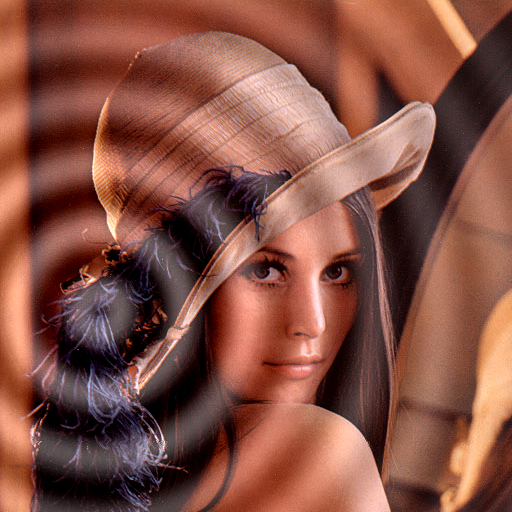
\includegraphics[width=0.3\textwidth]{imagenes/lenaONDA.jpg} \\
    \end{tabular}
     \end{center}
  \end{multicols}

\subsubsection{Implementación C}

Nuestra implementación en C es una traducción iterativa del mencionado algoritmo propuesto por la cátedra en el siguiente pseudocódigo:

\begin{algorithm}[H]
  \begin{algorithmic}[1]
    \FORALL{pixel ubicado en la posici'on $\mathbf{(x, y)}$}
      \STATE $d_x \gets x - x_0$
      \STATE
      \STATE $d_y \gets y - y_0$
      \STATE
      \STATE $d_{xy} \gets \sqrt{d_{x}^2+d_{y}^2}$
      \STATE
      \STATE $r \gets \frac{(d_{xy} - RADIUS)}{WAVELENGTH}$
      \STATE
      \STATE $a \gets \frac{1}{1 + (\frac{r}{TRAINWIDTH})^2 }$
      \STATE
      \STATE $t \gets ( r-floor(r) ) \cdot 2 \cdot \pi - \pi$
      \STATE
      \STATE $prof \gets a \cdot (t - \frac{t^3}{6}+\frac{t^5}{120}-\frac{t^7}{5040})$
      \STATE
      \STATE $pixel = prof \cdot 64 + I_{src}(x, y)$    
      \STATE
      \STATE $I_{dst}(x, y) = saturar(pixel)$
    \ENDFOR
  \end{algorithmic}
  \caption{$ondas (I_{src}, I_{dst}, x_0, y_0)$}
  \label{alg:ondas}
\end{algorithm}

\begin{itemize}
  \item $x_0$ e $y_0$ representan la posici'on donde est'a centrada la onda,
  \item $RADIUS$, $WAVELENGTH$ y $TRAINWIDTH$ son constantes que definen la 
  forma de la onda y
  \item $saturar(x)$ es una funci'on que retorna $0$ si $x$ es menor $0$, $255$
  si es mayor a $255$ y $x$ en cualquier otro caso.
\end{itemize}

\subsubsection{Implementación ASM}